\section{Fazit}

Das verfahrenstechnische Labor soll, zeitgemäß, digital transformiert werden. An der Stelle muss nochmals erwähnt werden, dass eine digitale Transformation ein Prozess und kein Projekt ist. Das Konzept 3.0, ohne Datenbankmanagementsystem (DBMS), sollte als Vorstufe des Konzept 4.0, mit DBMS, betrachtet werden. Das Konzept 3.0 ist eine Mindestanforderung für die digitale Transformation des verfahrenstechnischem Labors. Im folgenden werden die wünsche und Anforderung aus dem Kapitel \ref{sec:konzeptentwicklung} {\Hypatia Konzeptentwicklung für die Labordigitalisierung} aufgelistet. Die erfüllten Anforderungen werden mit einem Haken (\cmark) und die Anforderungen, die im Rahmen dieses Projekts nicht umgesetzt wurden, werden mit einem Kreuz (\xmark) markiert. Stichpunkte die Anmerkungen enthalten werden mit einem $\diamond$ gelabelt.

\begin{enumerate}[leftmargin = 1.2em, label = \textbullet , itemsep = 0.1em]
\item[\cmark] Das Konzept soll für das verfahrenstechnische Labor allgemeingültig sein.
\item[\cmark] Die \glqq digitalen Kompetenzen\grqq{} der Studierenden sollen maximiert werden, ohne die fachlichen Kompetenzen signifikant zu reduzieren, durch 


	\begin{enumerate}[leftmargin = 1.2em, label = -- , itemsep = 0.1em]
	\item[\cmark] ein Minimum an Automatisierung 
	\item[\cmark] Unter Automatisierung kann z.B.  die Manipulation von Daten, wie die Detektion von Ausreißer und dessen Entfernung, genaue Leitfäden in der Handhabung, die keine Fehler mehr zulassen o.ä., verstanden werden.
	\end{enumerate}
	
\item[\cmark] Der monetäre Aufwand soll minimal sein.
\item[\cmark] Möglichkeiten der Datenerfassung/Signalverarbeitung sollen eruiert werden. 
\item[\cmark] Die inkrementelle Implementation von Applikationen im Rahmen von Industrie 4.0 und Big Data (KI, Digital Twin etc.) soll tendenziell möglich sein.
	\begin{enumerate}[leftmargin = 1.2em, label = $\diamond$ , itemsep = 0.1em]
	\item Es wurden keine Schritte eingeleitet, die eine inkrementelle Implementation von Applikationen ausschließen.
	\end{enumerate}


\item[\cmark] Cloud Computing soll in Betracht gezogen werden.
	\begin{enumerate}[leftmargin = 1.2em, label = $\diamond$ , itemsep = 0.1em]
	\item Die Implementation eines Cloudservice (HAW Cloud) ist im Verlauf des Projekts nicht erfolgt. Laut einem ITSC-Mitarbeiter scheinen die HAW Richtlinien es	\textbf{derzeit} nicht zu gestatten, dass Kennungen an nicht humane Entitäten bzw. nicht natürliche Personen vergeben werden (siehe Anhang \ref{appendix:Cloudnutzung}).	Nicht humane Entitäten könnten die folgenden sein:
	 
		\begin{enumerate}[leftmargin = 1.2em, label = - , itemsep = 0.1em]
		\item Aggregate
		\item Maschinen
		\item Geräte
			\begin{enumerate}[leftmargin = 1.2em, label = $\circ$ , itemsep = 0.1em]
			\item HMI's 
			\item Sensoren
			\end{enumerate} 
		\end{enumerate}
	\end{enumerate}
	
	\begin{enumerate}[leftmargin = 1.2em, label = -- , itemsep = 0.1em]
	\item[\xmark] First Step: Speicherung der Rohdaten auf der HAW Cloud
		\begin{enumerate}[leftmargin = 1.2em, label = $\diamond$ , itemsep = 0.1em]
		\item Da die Nutzung der HAW Cloud möglich wäre, der Aufwand dem Nutzen jedoch nicht gerecht wird, wurde eine alternative Lösung entwickelt (siehe Protokoll im Anhang \ref{appendix:Cloudnutzung}). Als Alternative Lösung wurde ein Speicherlösung mittels lokalem Server vorgeschlagen.
		
		\end{enumerate} 
	\item[\xmark] Zukunftsvision, gemäß des Impulsvortrags zum Digitalisierungsfond: Amazon, Google, Microsoft Azure
	\end{enumerate}
	
\item[\xmark] Die gesamte Protokollierung der Studierenden soll in Zukunft digital sein.
\end{enumerate}

Ziel dieses Projekts ist es, Messwerte digital verfügbar zu machen und diese zu dokumentieren. Ein weiteres Ziel des Projekts ist es einen Wandel von der Versuchsdokumentation in Hardcopy, zu einer digitalen Dokumentation einzuleiten. Es ist anzumerken, dass dieses Konzept die \textbf{\emph{\underline{absolute Mindestanforderung}}} für den ersten Schritt in die digitale Transformation darstellt.\\

Im folgenden werden die Vorteile des Konzepts ohne eine Datenbank aufgelistet: 

\begin{itemize}
\singlespacing
\item Die Verfügbarkeit von digitalen Messwerten wird ermöglicht, 
\item Die Dokumentation der Versuchsrandbedingung, eingesetzte Rohstoffe etc. kann digital durchgeführt werden,
\item Die Verfügbarkeit der Versuchsdaten und Ergebnisse wird durch die Einführung eines elektronischen Labor Notebooks verbessert,
\item Versuchsbeobachtungen können direkt dem Zeitstempel zugeordnet werden.
\end{itemize}



%An dieser Stelle nun ein radikales dennoch wahres Beispiel aus meinem sechsten und siebten, Semester des erst Studiums, im Jahr 2017.
%
%\glqq Ich persönlich habe Vorlesungen, \textbf{\emph{\underline{mit Potential}}}, besuchen müssen, in denen \textbf{permanent} teilweise unlesbare Zeitungsartikel aus dem Jahr 19XX auf \textit{Over Head Projektoren} abgebildet wurden.\grqq{} Wie war das noch mit dem Stand der Technik? Das ist ebenfalls eine bis dato gelebte Mindestanforderung an der Hochschule! Eine harte, traurige, dennoch ware Tatsache!

Eine Mindestanforderung sollte jedoch kein Maßstab für eine Hochschule darstellen! Meines Erachtens nach unterliegt der Aufwand dem Nutzen der Konzeptrealisierung unter der Verwendung einer Datenbank im hohem Maße, aus den folgenden Gründen. 

Im akademischen Rahmen unterliegt der Aufwand, der Realisierung des zweiten Konzepts mit Datenbank, einen \textbf{großen} Mehrwert in Bezug auf das Verständnis und Lernerfolg der Studierenden. Die Datenbank könnte auch für den Laborbetrieb des Departments genutzt werden, wodurch sich möglicherweise organisatorische Vereinfachungen, wie z.B. Chemie- und Verfahrenstechniklagerverwaltung o.ä. realisieren lassen. Des Weiteren könnte die Datenbank für die verfahrenstechnische Forschung, Projekte im Rahmen der angewandten numerische Simulation uvm. genutzt werden.. Die \textbf{größte Hürde} für die Konzept 4.0 Realisierung könnte der \textbf{Changeprozess} sein, daher wurde der Punkt Changeprozess, in der Tabelle \ref{tab:konzept4.0_2} mit einem Dicken -- versehen.\\

In unserer agitierten Welt ist weder Platz für schwere Unternehmenstanker noch für träge Universitäten oder Hochschulen. In der Zeit der Globalisierung und digitalen Transformation ist Flexibilität und Vernetzung nicht nur eine hinreichende Forderung, sondern absolut notwendig. Unternehmen sollten sich Ihre Spitzenkräfte schaffen. Der Spruch, \glqq von der Berufsausbildung oder dem Studium braucht man am Ende des Tages maximal 15 \%\grqq , ist nicht tolerierbar sowie zu verantworten und doch ist es aus eigenen Erfahrungen Realität. Wie lange Überlebt ein Unternehmen welches 85 \% Ausschuss hat? Wenn durch diese Art des Paradigmenwechsels eine Ausschussreduktion auf bspw. 70 \% erfolgt, ist das ein immenser Fortschritt! 
In der Tabelle \ref{tab:konzept4.0} sind die Vor- und Nachteile des Konzepts 4.0 aufgelistet.\\




\begin{table}[p!]
\caption{Vor- und Nachteile des Konzeptentwurfs 4.0} \label{tab:konzept4.0_2}
\begin{center}
\begin{tabularx}{1\textwidth}{X|X}
Vorteile & Nachteile \\ \toprule \vspace{-1,5em}
\begin{itemize}[leftmargin=*,labelsep=-\mylen]
\item[+] Stand der Technik in der Industrie	/ Zeitgemäß 
\item[+] Nutzbar für Tätigkeiten außerhalb vom VT1 und VT2 Praktikum (Forschung, Organisatorisches 
wie 
\item[+] Lagerverwaltung, angewandte numerische Simulation	uvm.)
\item[+] wenn Cloudservicenutzung, dann Port\-folio\-software Kompatibilität des \mbox{Anbieters}
\item[+] Image/Professionalität (u.a. auch Anmerkungen von Bachelorabsolventen Ende 2020)
\item[+] ggf. mehr Kooperationsprojekte mit Unternehmen und Universitäten
\item[+] Kompetenzsteigerung der Hochschule und Absolventen
\item[+] interdisziplinäre Vernetzung/Projekte  (Industrie 4.0 $\equiv$ Vernetzung)
\item[+] gute Investigationsmöglichkeiten bei Produktabweichung bei konstanten Parametern $\rightarrow$ Studentenprojekte
\end{itemize}

&
\vspace{-1,5em}
\begin{itemize}[leftmargin=*,labelsep=-\mylen]
\item[--] Changeprozesse
\item[-] notwendiges Know-How erforderlich
\item[-] Aufwand der Erstellung der Datenbank
\item[-] Einrichtung automatischer Einspeisung der Sensordaten in die Datenbank
\item[-] Kosten könnten entstehen
\begin{itemize}[leftmargin=*,labelsep=-\mylen] 
\item[\textbullet] möglicherweise Sponsoring/Kooperation (als Gegenleistung Projekte o.ä) da Hochschule 
\item[\textbullet] geringe Datenmengen im vgl. zu Unternehmen $\rightarrow$ möglicherweise keine oder geringe Kosten
\end{itemize}

\end{itemize}
\end{tabularx}
\end{center}
\end{table}



Der Versuchsstand wurde mit geeigneter Sensorik aufgerüstet, um die kontinuierlichen Parameter Druck $p$ und Volumenstrom $\dot{V}$ zu erfassen. Die Signale des Drucksensors sind von 0~-~10~V und die des thermischen Massendurchflusssensors sind 4~-~20~mA. Eine digitale Erfassung der Festbett- bzw. Wirbelschichthöhe ist denkbar. Bei bedarf könnten bspw. geeignete optische, akustische, mechanische Entfernungsmesser, im Rahmen einer studentischen Projektarbeit, recherchiert und umgesetzt werden.



Die Idee, dass jeder Laboraccount eine eigene Kennung erhält, wodurch die Laborgeräte wie HMI's ein Cloudverzeichnis auf der HAW Cloud erhalten würden, ist derzeit nicht realisierbar. Die Idee, dass nicht humane Entitäten eine Kennung erhalten können, sollte in höheren Instanzen der HAW diskutiert werden, damit zukünftige Cloudlösungen HAW global realisiert werden können. Die Hochschule sollte das Ziel haben die Privatwirtschaft abzubilden. Das nicht humane Entitäten ein eigenes Kommunikationbsnetzwerk erhalten ist bereits Stand der Technik (siehe Abschnitt \ref{sec:bluetooth}). \textsl{•}




\addsec{Anhang}
%\addcontentsline{toc}{section}{Anhang}
\pagenumbering{roman}
%\vspace{-14pt}

\begin{table}[h!] % Parameter
\caption{Versuchsparameter der MVT Geräte und Anlagen} \label{tab:Versuchsparameter}
\begin{center}
\vspace{-14pt}
\begin{NiceTabular}{r|c|ccr|c|c}%[hvlines-except-corners=NW]
MVT Versuchsstände 	&	diskret 	& konti. & &MVT Versuchsstände 	&	diskret 	& konti. \\ \cline{1-3}  \cline{5-7}
\Block{1-7}{} 						& 						& &&&& \\[-13pt] \cline{1-3}  \cline{5-7}
Kuchenfiltration & &&& \makecell{Hochdruckhomo-\\genisator (HDH)}  \\ \cline{1-3}  \cline{5-7}
Gewicht 							& & \cmark && Fluid1 & \cmark &\\
Druck 								& & \cmark && Fluidvolumen1& \cmark &\\
Suspensionskonzentration 	& \cmark &&&Fluid2& \cmark & \\
Suspensionsvolumen 			& \cmark &&&Fluidvolumen2& \cmark &\\
Filterkuchendicke 				& \cmark &&&Disperer RPM& \cmark &   \\
Filterkuchendurchmesser		& \cmark &&&Dispersionsdauer& \cmark &\\
Filterkuchenvolumen 			& \cmark &&&Druck& \cmark &\\
Filterkuchenfeuchtegehalt 	& \cmark &&&HDH Dauer& \cmark &\\
Filternutschen Nr. 				& \cmark &&&Temperatur& \cmark & \\
Filterporösität 					& \cmark &&&Partikelgrößenverteilung& \cmark & \\
\Block{1-7}{} 						& 						& &&&& \\

Gas-Feststoff Wirbelschicht & &&& ZickZack Sichten && \\  \cline{1-3}  \cline{5-7}
$\mathrm{Volumenstrom_{Luft}}$ & & \cmark && Feststoff & \cmark & \\
Druck & & \cmark && Gesamtmasse & \cmark & \\
Festbetthöhe & \cmark & && Masse Grobgut&\cmark &\\
Schüttgutmasse & \cmark & && Masse Feingut&& \\
Partikeldichte & \cmark & && \makecell{ Vibrationsintensität der\\ Vibrationsförderung} & \cmark &\\
Wirbelschichthöhe = f(p) & \cmark &  \cmark && Volumenstrom & \cmark &  \\
Wirbelschichtporösität = f(p) & \cmark &  \cmark && Förderklappenstellung & \cmark & \\
Sauterdurchmesser & \cmark & \Block{1-5}{} &&& \\
Festbettporösität & \cmark & \Block{1-5}{} &&&& \\
\Block{1-7}{} 				& 						& &&&& \\

Rührversuch &&&& Walzenmühle && \\  \cline{1-3} \cline{5-7}
Fluid & \cmark  &&& Feststoff & \cmark & \\
Fluiddichte & \cmark &&& Masse & \cmark & \\
dynamische Viskosität & \cmark &&& Walzengeometrie (Profil) & \cmark & \\
Rührer & \cmark &&& Walzenspalt & \cmark & \\
Rührereintauchtiefe & \cmark &&& Umfangsgeschwindigkeit & \cmark & \\
Strombrecher & \cmark & \Block{1-5}{} &&&& \\
RPM & \cmark & \Block{1-5}{} &&&& \\
Drehmoment &  & \cmark & \Block{1-4}{} &&& \\

%Kuchenfiltration & \xmark 			& \textcolor{red}{\xmark} \\

\end{NiceTabular}
\end{center}
\end{table}

%%==================================================================================
%\newpage
%\begin{figure}[]
%\centering
%\includegraphics[width=0.8\textwidth]{Bilder/speicherbedarf_ascii-binär.jpg}
%\caption{Speicherbedarfsvergleich ASCII/binär \cite[S. 44]{speicherbedarf_vergleich_binär-ascii}}
%\label{fig:speicherbedarf_vergleich}
%\end{figure}

\paragraph*{Ergänzung des Abschnitts Dehnungsresistive Sensoren}

Die Drucksensoren mittels DMS sind dehnungsresistive Sensoren. Das Messprinzip beruht auf die Änderung des elektrischen Widerstandes R, eines elektrisch leitenden Werkstoffs, als Folge einer mechanischen Verformung. Ein zylinderförmiger Werkstoff, charakterisiert durch die Ausgangslänge $l_0$, Ausgangsquerschnitt $A_0$ und dem spezifischem elektrischem Widerstand $\rho_{el}$, hat einen elektrischen Widerstand R gemäß folgender Gleichung \cite[S. 4 ff.]{Wolff2016}:

\begin{align}
R=\rho_{el} \cdot \frac{l_0}{A_0}
\end{align}

Um die relative Widerstandsänderung $\Delta R / R$ zu berechnen wird das totale Differenzial (Gleichung \ref{eq:totaldif_dms}) aus Gleichung \ref{eq:zyl_wiederstand} gebildet.


\begin{align}  
\label{eq:totaldif_dms}
	dR &=\frac{\partial R}{\partial \rho_{el}} \: d\rho_{el}+\frac{\partial R}{\partial l_0} \: dl_0+\frac{\partial R}{\partial A} \: dA \\[1em]
		&= \frac{l_0}{A} ~ d\rho_{el} + \frac{\rho_{el}}{A} \: dl_0 - \frac{\rho_{el} \cdot l_0}{A^2} \: dA \\[1em]
		&= R \cdot ( \frac{d\rho_{el}}{\rho_{el}} + \frac{dl_0}{l_0} - \frac{dA}{A} )
\end{align}


Ersetzt man das Infinitisimal $d$ durch eine eine größere Schrittweite $\Delta$, unter der Bedingung dass $\Delta \rho \ll \rho,\, \Delta l_0 \ll l_0, \Delta A \ll A$, dann erhält man Gleichung \ref{eq:delta}. 

\begin{align}
% \label{eq:delta}
\frac{\Delta R}{R} = \frac{\Delta \rho_{el}}{\rho_{el}} + \frac{\Delta l}{l_0} - \frac{\Delta A}{A_0}
\end{align}

Die geometrische Verformung wird durch die beiden letzten Terme repräsentiert. Die Dehnung $\varepsilon$ ersetzt $\Delta l / l_0$ und der Term $\Delta A/A$ wird durch die Querkontraktion ($\varepsilon_Q = \frac{\Delta D}{D_0} = - \nu \cdot \varepsilon$), mit der Querkontraktionszahl (Poisson-Konstante) $\nu$, beschrieben und führt zu der Lösung der Gleichung (\ref{eq:querkontraktion}) .

%\begin{equation}
 \begin{align}
\frac{\Delta A}{A} &= \frac{\frac{\pi}{4} \cdot \bigl((D+\Delta D)^2-D^2 \bigr)}{\frac{\pi}{4} \cdot D^2}  \\[0.7em]
&= \frac{2D \cdot \Delta D + (\Delta D)^2}{D^2} \\[0.7em]
&\approx \frac{2 \Delta D}{D} \\[0.7em]
&=2\varepsilon_Q = -2 \cdot \nu \cdot \varepsilon %\label{eq:querkontraktion}
\end{align}
%\end{equation}

Durch Einsetzen der Gleichung (\ref{eq:querkontraktion}) und der Dehnung $\varepsilon$ in die Gleichung (\ref{eq:delta}) erhält man:

\begin{align}
\label{eq:wiederstand_substi}
\frac{\Delta R}{R} =(1+2 \cdot \nu) \cdot \varepsilon + \frac{\Delta \rho_{el}}{\rho_{el}}
\end{align}

Der Term $\frac{\Delta \rho_{el}}{\rho_{el}}$ ist der sog. \glqq piezoresistive Effekt\grqq , der bei metallischen Leitern vernachlässigbar ist, jedoch bei Halbleitern überwiegt. 



\begin{figure}[h!]
\centering
\caption{Kenndaten von Kapazitiven und piezoresistenten Drucksensoren \cite[S. 472 ff.]{Tränkler2015}}
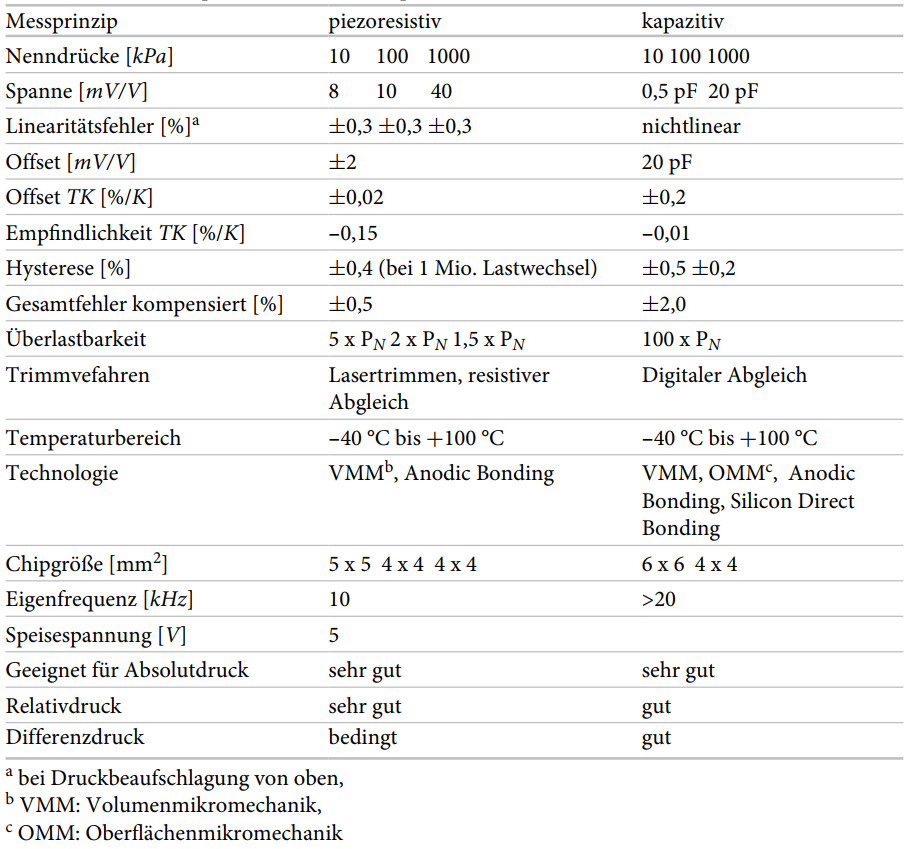
\includegraphics[width=1\textwidth]{Bilder/piezo_kapa.jpg}
\label{tab:piezo_kapa} 
\end{figure}


\begin{minipage}[][][t]{1\textwidth}
\centering
\includegraphics[width=0.8\textwidth]{Bilder/speicherbedarf_ascii-binär.jpg}
\captionof{figure}{Speicherbedarfsvergleich ASCII/binär \cite[S. 44]{speicherbedarf_vergleich_binär-ascii}}
\label{fig:speicherbedarf_vergleich}
\end{minipage}

%\newpage
\begin{figure}[ph!]
\centering
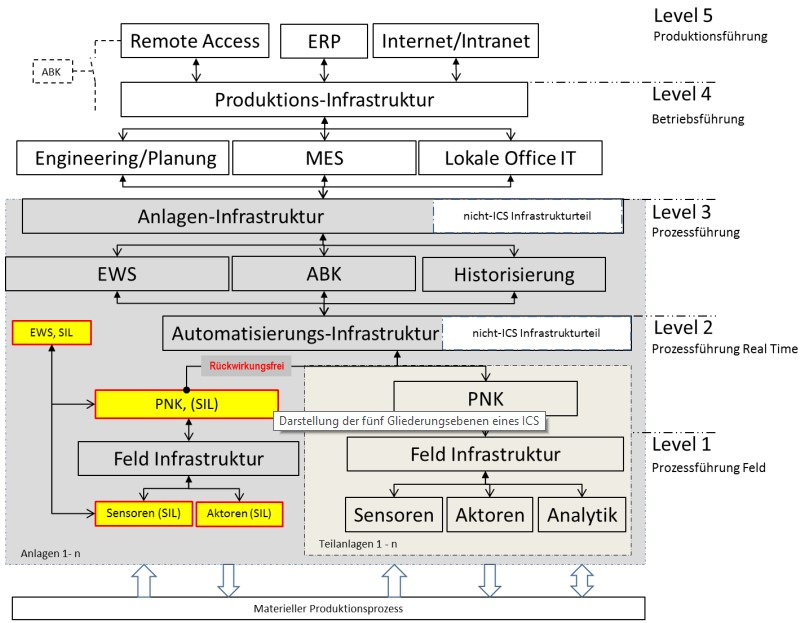
\includegraphics[width=1\textwidth]{Bilder/Hierarchische_Gliederung_eines_ICS_gemäß_ICS-Kompendium.jpg}
\vspace{0em}
\captionof{figure}{Hierarchische Gliederung eines ICS, gemäß ICS-Kompendium des Bundesamtes für Sicherheit in der Informationstechnik \cite[S. 18]{ics_kompendium}}\label{fig:Hierarchische_Gliederung_gem_ICS}
\end{figure}

\begin{figure}[ph!]
\centering 
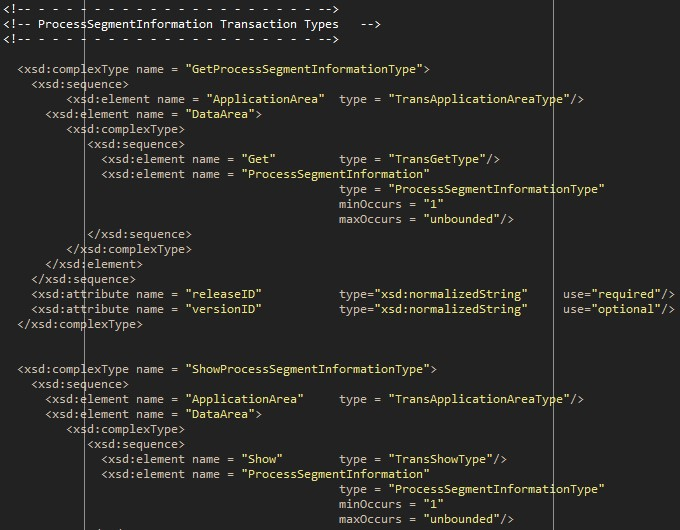
\includegraphics[width=1\textwidth]{Bilder/processsegmentinformationtype.jpg}
\caption[]{Ausschnitt der \textit{ProcessSegment} XSD der B2MML-V0600-ProcessSegment.xsd}
\label{fig:processsegment}
\end{figure}


\newpage



\section*{Machine Learning}

Einige Algorithmen müssen angelernt werden (\textit{engl. \textbf{supervised} or \textbf{semi-supervised}}), z.B. das vom Google-Brain-Team entwickelte open-source Modell, Tensor Flow \cite{tensorflow_framework}. Andere werden nicht angelernt und generieren Ihren Algorithmus autonom (\textit{engl. \textbf{unsupervised}}; vgl. \ref{fig:supervised_machinelearning} im Anhang). \textbf{Supervised Learning}  (vgl. Abbildung \ref{fig:supervised_machinelearning} im Anhang) bedeutet, dass Datensätze vorgegeben werden und zugleich deren Lösung bzw. Klassifizierungen. Anhand des dadurch generierten Algorithmus werden unbekannte Datensätze klassifiziert. Je nach verwendetem Algorithmus können Klassifizierungen binär wie Spam, nicht Spam; Mann, Frau oder Multi-Class-Klassifizierungen, wie z.B. Porsche, Mercedes, VW, .... sein. \textbf{Semi-Supervised Learning} Algorithmen verändern ihren angelernt Algorithmen, bzw. können Ihren Algorithmus, anhand der unvalidierten Daten, die sie nach dem anlernen erhalten, optimieren. KI Algorithmen benötigen große, Datenmengen. Einfache KI's benötigen zusätzlich strukturierte Daten, damit ist die Verfügbarkeit der Daten in Datenbanken gemeint. Die neusten, komplexen \cite{unstrukturierte_daten_ki} maschine learning Algorithmen können auch mit unstrukturierten Daten verwertbare Ergebnisse generieren, doch es gilt stets GIGO, \glqq garbage in, garbage out!\grqq{} Die Güte der Ergebnisse einer KI wird durch die Güte der Ausgangsdaten bestimmt, demnach ist die Wahrscheinlichkeit mit strukturierten Daten ein sinnvolles, aussagekräftiges Ergebnis zu erzielen wahrscheinlich höher.
Es existiert noch eine vierte Kategorie, die \textbf{Reinforced Learning} Algorithmen. Diese Algorithmen unterscheiden sich von den unsupervised Algorithmen in der Art, dass sie mit einer Umgebung (\textit{engl. environment}) interagieren und dadurch lernen \cite[S. 15 f.]{machine_learning_kompakt}. Als Beispiele können Roboter oder KI in einem Spiel wie Schach, Go (die asiatische, komplexere Schachvariante), aber auch in Videospielen genannt werden \cite{reinforced_learning_go}.

Zu den \textbf{Unsupervised Lerning} Algorithmen zählen z.B. die Regressionsanalyse oder die k-mean Clusteranalyse \cite[S. 114]{machine_learning_kompakt}. Um bei \textbf{supervised} oder \textbf{semi-supervised} verwertbare Ergebnisse zu erhalten, wird in vielen Anwendungsfällen eine \glqq große\grqq{} Datenbasis benötigt. Des Weiteren ist die Güte der Daten entscheidend für die Güte der Ergebnisse. Weniger komplexe KI Algorithmen benötigen strukturierte Daten, wofür sich Datenbankmanagementsysteme (DBMS) auszeichnen.\\

   \begin{figure}[b!] % 
%\captionsetup{position=top}
\centering
     \subfloat[Supervised Machine Learning][Supervised Machine Learning \label{fig:supervised_machinelearning}]{%
       \hspace{0em}
       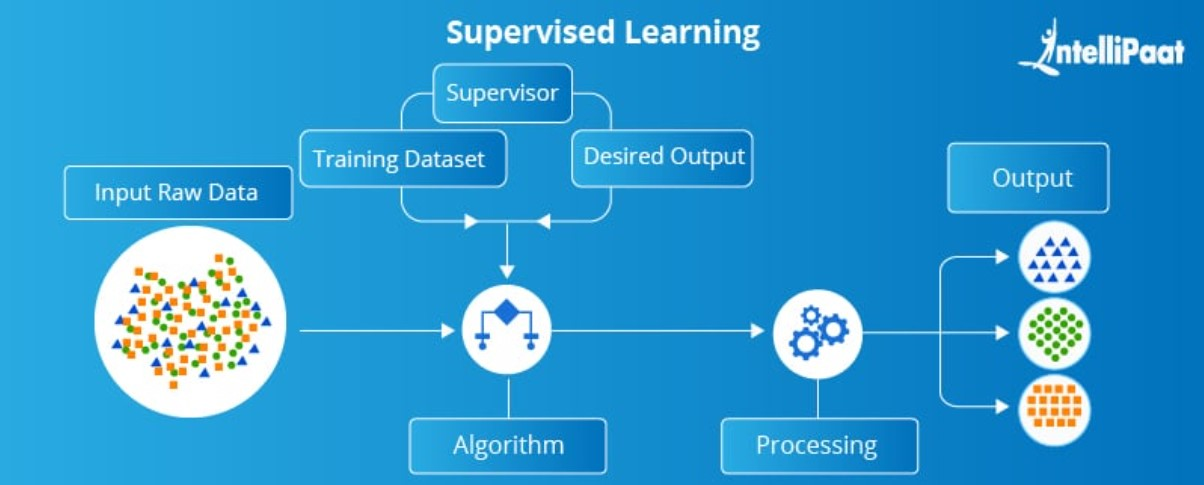
\includegraphics[width=0.8\textwidth]{Bilder/supervised.jpg}
            }
    \phantomcaption
    \vspace{1em}
    \ContinuedFloat
\captionsetup{position=bottom}
\subfloat[Unsupervised Machine Learning][Unsupervised Machine Learning \label{fig:unsupervised_machinelearning}]{%
       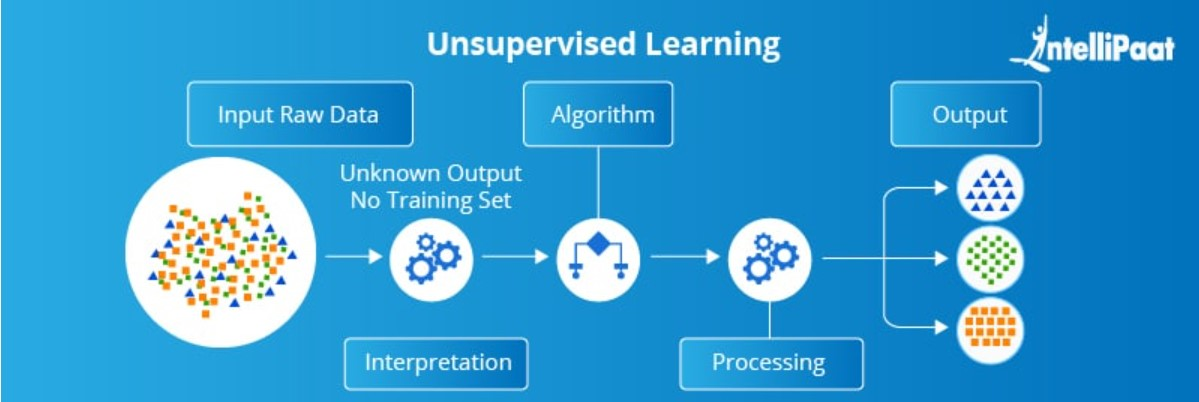
\includegraphics[width=0.8\textwidth]{Bilder/unsupervised.jpg}
       }
        \phantomcaption
    \vspace{1em}
    \ContinuedFloat
\captionsetup{position=bottom}
\subfloat[Reinforced Machine Learning][Reinforced Machine Learning \label{fig:reinforced_machinelearning}]{%
       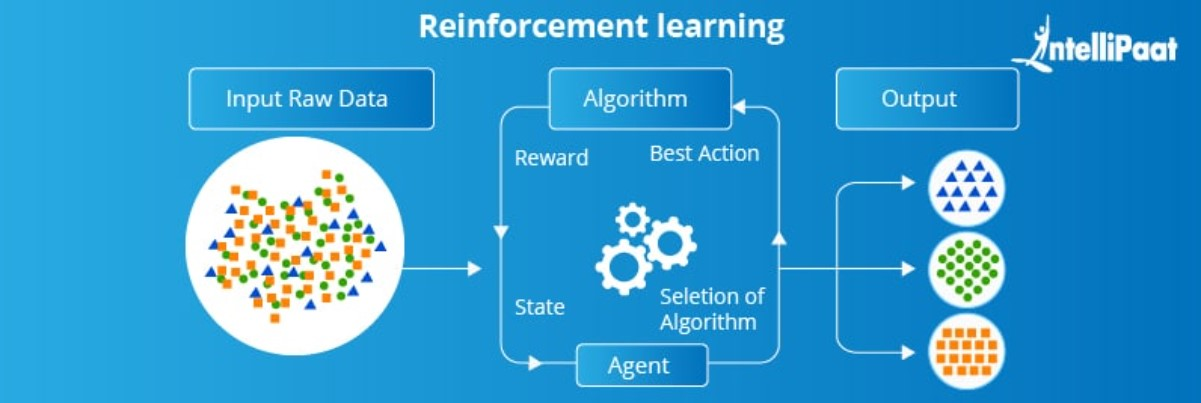
\includegraphics[width=0.8\textwidth]{Bilder/reinforced.jpg}
       }
\caption[]{Machine Learning \cite{intellipaat_unsupervised}}
\label{}
   \end{figure}
   
\begin{sidewaysfigure}
\caption[]{Dehnungsresistive Sensoren}\label{fig:metall_halbleiter_dms} \vspace{1em}
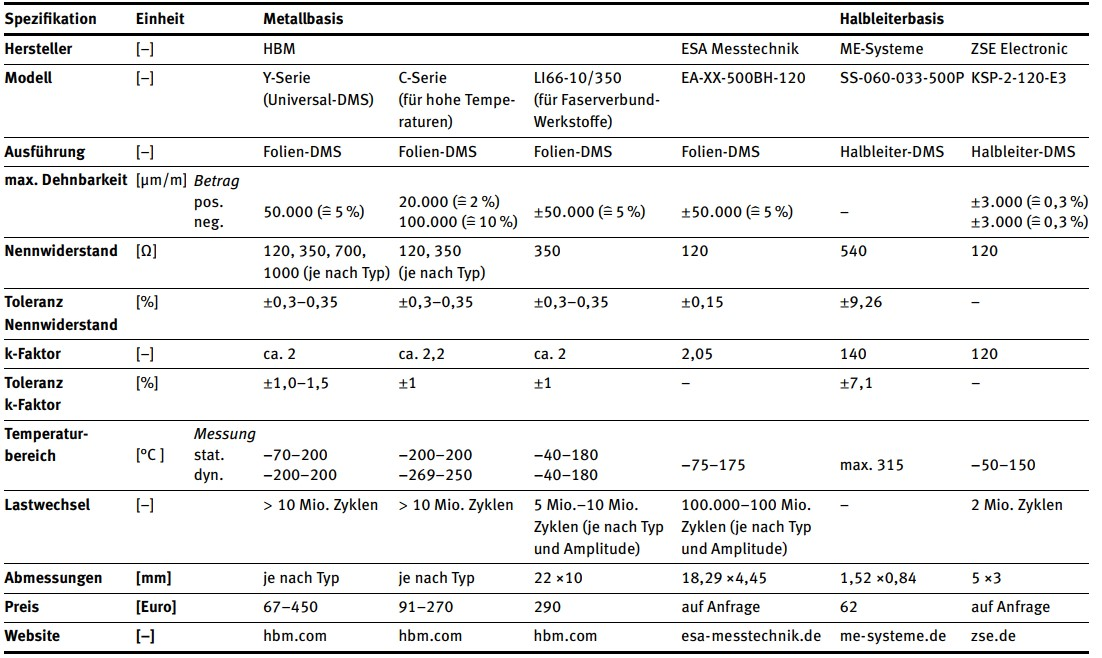
\includegraphics[width=1\textwidth]{Bilder/Metall_Halbleiter_dms.jpg}
\vspace{0em}
 \end{sidewaysfigure}
 

 \begin{figure}[h!] %[htbp!] 
 \centering
 \includegraphics[width=0.8\textwidth]{Bilder/schwebekörperkennline_ms-0_6585g.jpg}
 \vspace{0em}
  \caption[]{Schwebekörperdurchflussmesser (m=0,6585~g) mit einer Messspanne von 0,185~bis~5~l/min, zzgl. Approximationsfunktionen der Kennlinie}\label{fig:kleiner_skdm}
 \end{figure} 
 
 \begin{figure}[h!] %[htbp!] 
 \centering
 \includegraphics[width=0.8\textwidth]{Bilder/schwebekörperkennline_ms-2_225g.jpg}
 \vspace{0em}
  \caption[]{Schwebekörperdurchflussmesser (m=2,225~g) mit einer Messspanne von 1,86~l/min~bis~50~l/min, zzgl. Approximationsfunktionen der Kennlinie}\label{fig:grosser_skdm}
 \end{figure}
 
 \begin{figure}[h!] %[htbp!] 
 \centering
 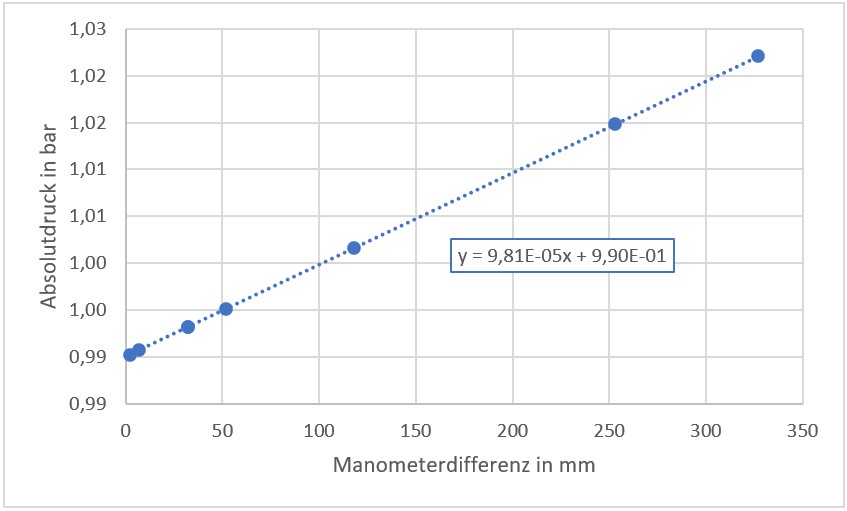
\includegraphics[width=0.8\textwidth]{Bilder/manometer_plus_0-99_bar_atm.jpg}
 \vspace{0em}
  \caption[]{Manometerkennline; Druckdifferenz zzgl. 0,99~bar, laut digitalem Drucksensor am 17.12.20, um 13:02~Uhr}\label{fig:manometer_kennlinie}
 \end{figure}
 


\begin{figure}[h!] %[htbp!] 
\centering
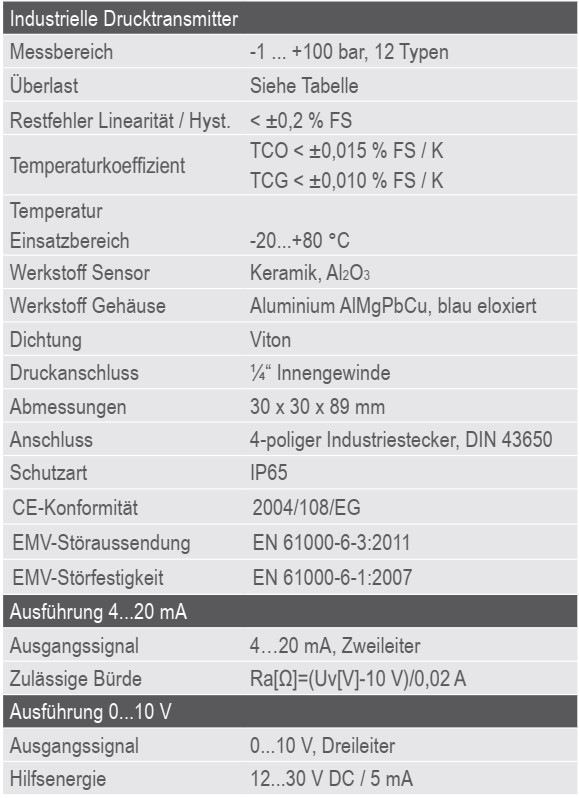
\includegraphics[width=0.5\textwidth]{Bilder/drtr-technische-Daten.jpg}
\vspace{0em}
 \caption[]{Technische Daten des DRTR-AL-10V-RV1 Drucksensors, (dem technischen Datenblatt entnommen \cite{BTTG2021})}\label{fig:BTTG2021}
\end{figure}

%\includepdf[scale=0.8,pages=16,pagecommand={}\label{appendix:bslut}]{mypages}
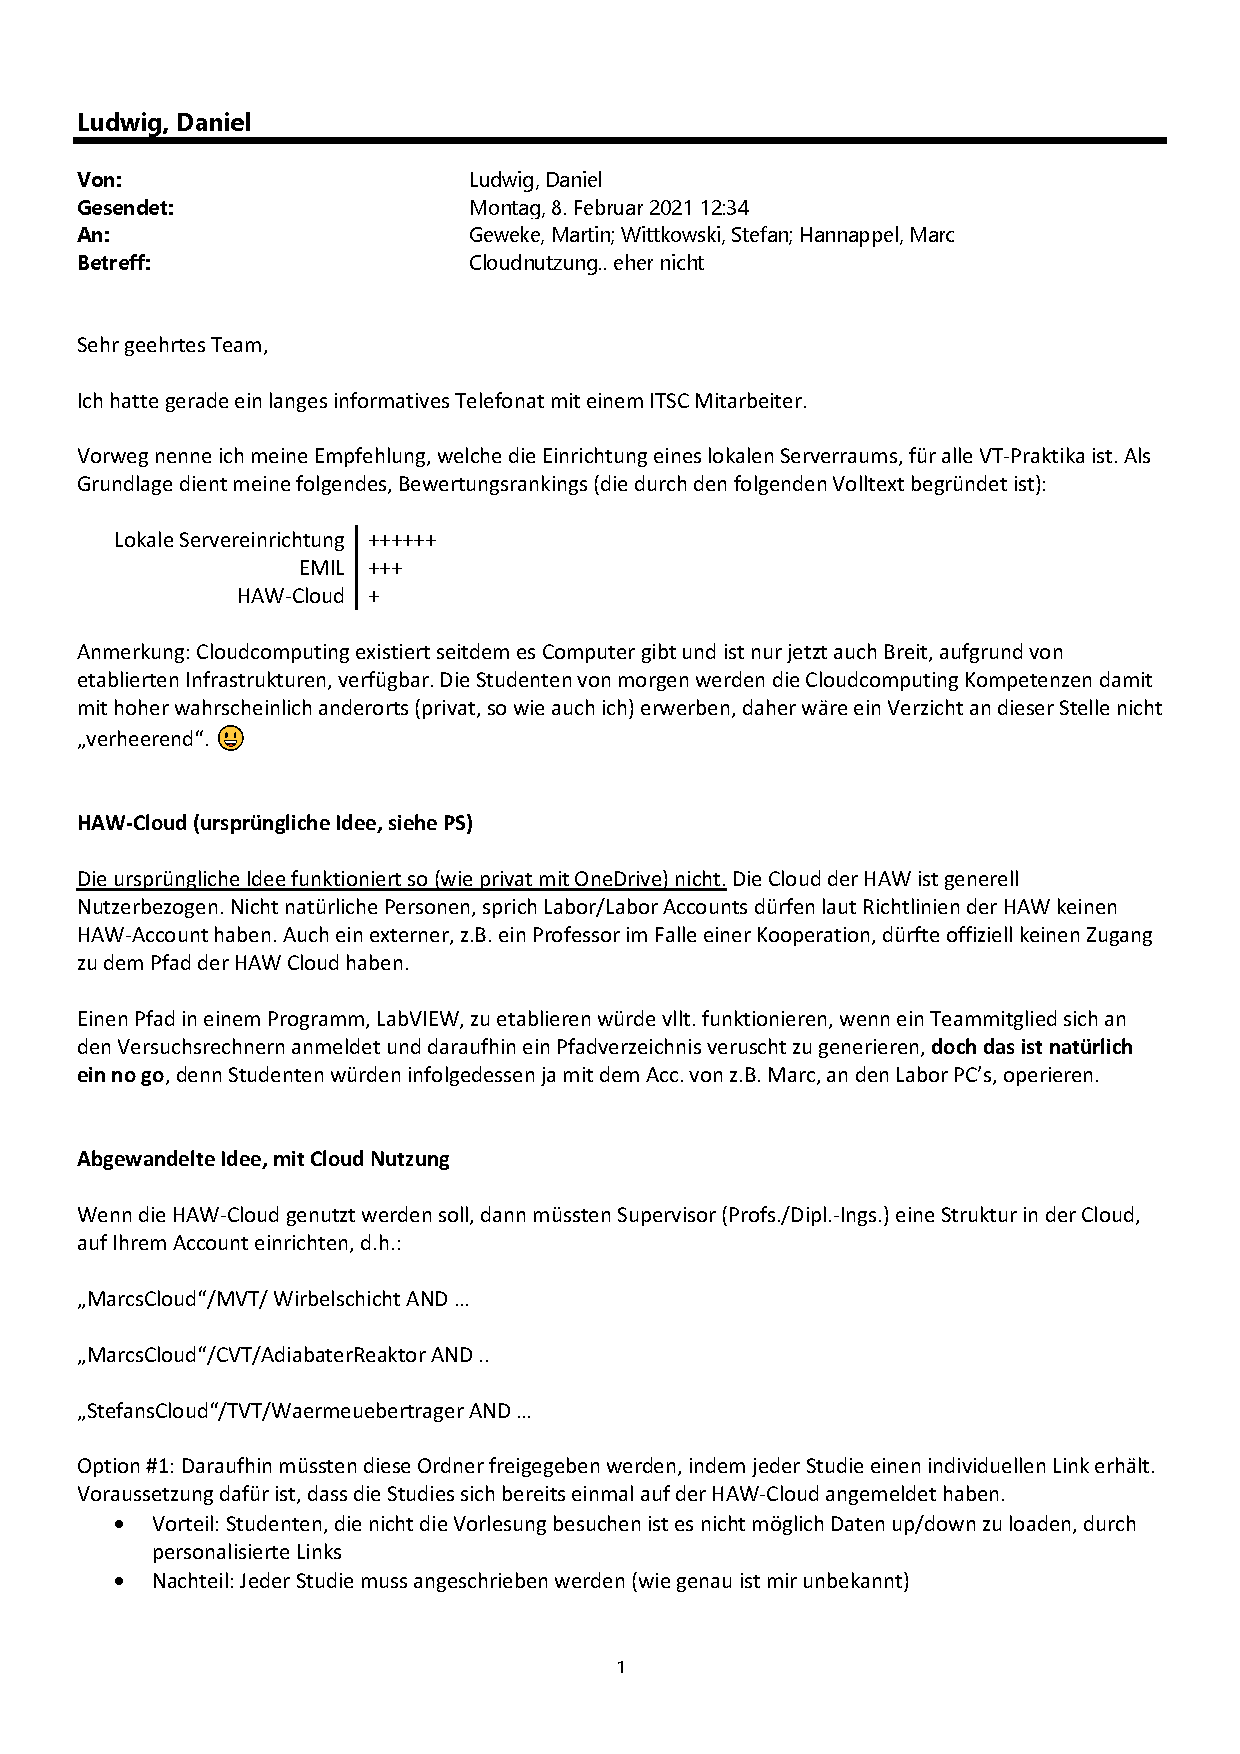
\includepdf[scale=0.8,pages=-,pagecommand={\label{appendix:Cloudnutzung}}]{Cloudnutzung.pdf}


%%==================================================================================
%\begin{center}
\begin{longtable}{llllll}
\caption{ASCII-Table \cite{ascii}} \label{ascii_table} \\
\vspace{0em} \\

\rowcolor[HTML]{FCFCFC} 
{\color[HTML]{404040} \textbf{Decimal}} & {\color[HTML]{404040} \textbf{Binary}} & {\color[HTML]{404040} \textbf{Octal}} & {\color[HTML]{404040} \textbf{Hexadec.}} & {\color[HTML]{404040} \textbf{Symbol}}    & {\color[HTML]{404040} \textbf{Description}}                  \\
\endfirsthead
%
\endhead
%
\rowcolor[HTML]{F3F6F6} 
{\color[HTML]{404040} 0}                & {\color[HTML]{404040} 0}               & {\color[HTML]{404040} 0}              & {\color[HTML]{404040} 0}                    & {\color[HTML]{404040} NUL}                & {\color[HTML]{404040} Null char}                             \\
\rowcolor[HTML]{FCFCFC} 
{\color[HTML]{404040} 1}                & {\color[HTML]{404040} 1}               & {\color[HTML]{404040} 1}              & {\color[HTML]{404040} 1}                    & {\color[HTML]{404040} SOH}                & {\color[HTML]{404040} Start of Heading}                      \\
\rowcolor[HTML]{F3F6F6} 
{\color[HTML]{404040} 2}                & {\color[HTML]{404040} 10}              & {\color[HTML]{404040} 2}              & {\color[HTML]{404040} 2}                    & {\color[HTML]{404040} STX}                & {\color[HTML]{404040} Start of Text}                         \\
\rowcolor[HTML]{FCFCFC} 
{\color[HTML]{404040} 3}                & {\color[HTML]{404040} 11}              & {\color[HTML]{404040} 3}              & {\color[HTML]{404040} 3}                    & {\color[HTML]{404040} ETX}                & {\color[HTML]{404040} End of Text}                           \\
\rowcolor[HTML]{F3F6F6} 
{\color[HTML]{404040} 4}                & {\color[HTML]{404040} 100}             & {\color[HTML]{404040} 4}              & {\color[HTML]{404040} 4}                    & {\color[HTML]{404040} EOT}                & {\color[HTML]{404040} End of Transmission}                   \\
\rowcolor[HTML]{FCFCFC} 
{\color[HTML]{404040} 5}                & {\color[HTML]{404040} 101}             & {\color[HTML]{404040} 5}              & {\color[HTML]{404040} 5}                    & {\color[HTML]{404040} ENQ}                & {\color[HTML]{404040} Enquiry}                               \\
\rowcolor[HTML]{F3F6F6} 
{\color[HTML]{404040} 6}                & {\color[HTML]{404040} 110}             & {\color[HTML]{404040} 6}              & {\color[HTML]{404040} 6}                    & {\color[HTML]{404040} ACK}                & {\color[HTML]{404040} Acknowledgement}                       \\
\rowcolor[HTML]{FCFCFC} 
{\color[HTML]{404040} 7}                & {\color[HTML]{404040} 111}             & {\color[HTML]{404040} 7}              & {\color[HTML]{404040} 7}                    & {\color[HTML]{404040} BEL}                & {\color[HTML]{404040} Bell}                                  \\
\rowcolor[HTML]{F3F6F6} 
{\color[HTML]{404040} 8}                & {\color[HTML]{404040} 1000}            & {\color[HTML]{404040} 10}             & {\color[HTML]{404040} 8}                    & {\color[HTML]{404040} BS}                 & {\color[HTML]{404040} Back Space}                            \\
\rowcolor[HTML]{FCFCFC} 
{\color[HTML]{404040} 9}                & {\color[HTML]{404040} 1001}            & {\color[HTML]{404040} 11}             & {\color[HTML]{404040} 9}                    & {\color[HTML]{404040} HT}                 & {\color[HTML]{404040} Horizontal Tab}                        \\
\rowcolor[HTML]{F3F6F6} 
{\color[HTML]{404040} 10}               & {\color[HTML]{404040} 1010}            & {\color[HTML]{404040} 12}             & {\color[HTML]{404040} 0A}                   & {\color[HTML]{404040} LF}                 & {\color[HTML]{404040} Line Feed}                             \\
\rowcolor[HTML]{FCFCFC} 
{\color[HTML]{404040} 11}               & {\color[HTML]{404040} 1011}            & {\color[HTML]{404040} 13}             & {\color[HTML]{404040} 0B}                   & {\color[HTML]{404040} VT}                 & {\color[HTML]{404040} Vertical Tab}                          \\
\rowcolor[HTML]{F3F6F6} 
{\color[HTML]{404040} 12}               & {\color[HTML]{404040} 1100}            & {\color[HTML]{404040} 14}             & {\color[HTML]{404040} 0C}                   & {\color[HTML]{404040} FF}                 & {\color[HTML]{404040} Form Feed}                             \\
\rowcolor[HTML]{FCFCFC} 
{\color[HTML]{404040} 13}               & {\color[HTML]{404040} 1101}            & {\color[HTML]{404040} 15}             & {\color[HTML]{404040} 0D}                   & {\color[HTML]{404040} CR}                 & {\color[HTML]{404040} Carriage Return}                       \\
\rowcolor[HTML]{F3F6F6} 
{\color[HTML]{404040} 14}               & {\color[HTML]{404040} 1110}            & {\color[HTML]{404040} 16}             & {\color[HTML]{404040} 0E}                   & {\color[HTML]{404040} SO}                 & {\color[HTML]{404040} Shift Out / X-On}                      \\
\rowcolor[HTML]{FCFCFC} 
{\color[HTML]{404040} 15}               & {\color[HTML]{404040} 1111}            & {\color[HTML]{404040} 17}             & {\color[HTML]{404040} 0F}                   & {\color[HTML]{404040} SI}                 & {\color[HTML]{404040} Shift In / X-Off}                      \\
\rowcolor[HTML]{F3F6F6} 
{\color[HTML]{404040} 16}               & {\color[HTML]{404040} 10000}           & {\color[HTML]{404040} 20}             & {\color[HTML]{404040} 10}                   & {\color[HTML]{404040} DLE}                & {\color[HTML]{404040} Data Line Escape}                      \\
\rowcolor[HTML]{FCFCFC} 
{\color[HTML]{404040} 17}               & {\color[HTML]{404040} 10001}           & {\color[HTML]{404040} 21}             & {\color[HTML]{404040} 11}                   & {\color[HTML]{404040} DC1}                & {\color[HTML]{404040} Device Control 1 (oft.XON)}            \\
\rowcolor[HTML]{F3F6F6} 
{\color[HTML]{404040} 18}               & {\color[HTML]{404040} 10010}           & {\color[HTML]{404040} 22}             & {\color[HTML]{404040} 12}                   & {\color[HTML]{404040} DC2}                & {\color[HTML]{404040} Device Control 2}                      \\
\rowcolor[HTML]{FCFCFC} 
{\color[HTML]{404040} 19}               & {\color[HTML]{404040} 10011}           & {\color[HTML]{404040} 23}             & {\color[HTML]{404040} 13}                   & {\color[HTML]{404040} DC3}                & {\color[HTML]{404040} Device Control 3 (oft.XOFF)}           \\
\rowcolor[HTML]{F3F6F6} 
{\color[HTML]{404040} 20}               & {\color[HTML]{404040} 10100}           & {\color[HTML]{404040} 24}             & {\color[HTML]{404040} 14}                   & {\color[HTML]{404040} DC4}                & {\color[HTML]{404040} Device Control 4}                      \\
\rowcolor[HTML]{FCFCFC} 
{\color[HTML]{404040} 21}               & {\color[HTML]{404040} 10101}           & {\color[HTML]{404040} 25}             & {\color[HTML]{404040} 15}                   & {\color[HTML]{404040} NAK}                & {\color[HTML]{404040} Negative Acknowledgement}              \\
\rowcolor[HTML]{F3F6F6} 
{\color[HTML]{404040} 22}               & {\color[HTML]{404040} 10110}           & {\color[HTML]{404040} 26}             & {\color[HTML]{404040} 16}                   & {\color[HTML]{404040} SYN}                & {\color[HTML]{404040} Synchronous Idle}                      \\
\rowcolor[HTML]{FCFCFC} 
{\color[HTML]{404040} 23}               & {\color[HTML]{404040} 10111}           & {\color[HTML]{404040} 27}             & {\color[HTML]{404040} 17}                   & {\color[HTML]{404040} ETB}                & {\color[HTML]{404040} End of Transmit Block}                 \\
\rowcolor[HTML]{F3F6F6} 
{\color[HTML]{404040} 24}               & {\color[HTML]{404040} 11000}           & {\color[HTML]{404040} 30}             & {\color[HTML]{404040} 18}                   & {\color[HTML]{404040} CAN}                & {\color[HTML]{404040} Cancel}                                \\
\rowcolor[HTML]{FCFCFC} 
{\color[HTML]{404040} 25}               & {\color[HTML]{404040} 11001}           & {\color[HTML]{404040} 31}             & {\color[HTML]{404040} 19}                   & {\color[HTML]{404040} EM}                 & {\color[HTML]{404040} End of Medium}                         \\
\rowcolor[HTML]{F3F6F6} 
{\color[HTML]{404040} 26}               & {\color[HTML]{404040} 11010}           & {\color[HTML]{404040} 32}             & {\color[HTML]{404040} 1A}                   & {\color[HTML]{404040} SUB}                & {\color[HTML]{404040} Substitute}                            \\
\rowcolor[HTML]{FCFCFC} 
{\color[HTML]{404040} 27}               & {\color[HTML]{404040} 11011}           & {\color[HTML]{404040} 33}             & {\color[HTML]{404040} 1B}                   & {\color[HTML]{404040} ESC}                & {\color[HTML]{404040} Escape}                                \\
\rowcolor[HTML]{F3F6F6} 
{\color[HTML]{404040} 28}               & {\color[HTML]{404040} 11100}           & {\color[HTML]{404040} 34}             & {\color[HTML]{404040} 1C}                   & {\color[HTML]{404040} FS}                 & {\color[HTML]{404040} File Separator}                        \\
\rowcolor[HTML]{FCFCFC} 
{\color[HTML]{404040} 29}               & {\color[HTML]{404040} 11101}           & {\color[HTML]{404040} 35}             & {\color[HTML]{404040} 1D}                   & {\color[HTML]{404040} GS}                 & {\color[HTML]{404040} Group Separator}                       \\
\rowcolor[HTML]{F3F6F6} 
{\color[HTML]{404040} 30}               & {\color[HTML]{404040} 11110}           & {\color[HTML]{404040} 36}             & {\color[HTML]{404040} 1E}                   & {\color[HTML]{404040} RS}                 & {\color[HTML]{404040} Record Separator}                      \\
\rowcolor[HTML]{FCFCFC} 
{\color[HTML]{404040} 31}               & {\color[HTML]{404040} 11111}           & {\color[HTML]{404040} 37}             & {\color[HTML]{404040} 1F}                   & {\color[HTML]{404040} US}                 & {\color[HTML]{404040} Unit Separator}                        \\
\rowcolor[HTML]{F3F6F6} 
{\color[HTML]{404040} 32}               & {\color[HTML]{404040} 100000}          & {\color[HTML]{404040} 40}             & {\color[HTML]{404040} 20}                   & {\color[HTML]{404040} SPACE}              & {\color[HTML]{404040} Space}                                 \\
\rowcolor[HTML]{FCFCFC} 
{\color[HTML]{404040} 33}               & {\color[HTML]{404040} 100001}          & {\color[HTML]{404040} 41}             & {\color[HTML]{404040} 21}                   & {\color[HTML]{404040} !}                  & {\color[HTML]{404040} Exclamation mark}                      \\
\rowcolor[HTML]{F3F6F6} 
{\color[HTML]{404040} 34}               & {\color[HTML]{404040} 100010}          & {\color[HTML]{404040} 42}             & {\color[HTML]{404040} 22}                   & {\color[HTML]{404040} “}                  & {\color[HTML]{404040} Double quotes (or speech marks)}       \\
\rowcolor[HTML]{FCFCFC} 
{\color[HTML]{404040} 35}               & {\color[HTML]{404040} 100011}          & {\color[HTML]{404040} 43}             & {\color[HTML]{404040} 23}                   & {\color[HTML]{404040} \#}                 & {\color[HTML]{404040} Number}                                \\
\rowcolor[HTML]{F3F6F6} 
{\color[HTML]{404040} 36}               & {\color[HTML]{404040} 100100}          & {\color[HTML]{404040} 44}             & {\color[HTML]{404040} 24}                   & {\color[HTML]{404040} \$}                 & {\color[HTML]{404040} Dollar}                                \\
\rowcolor[HTML]{FCFCFC} 
{\color[HTML]{404040} 37}               & {\color[HTML]{404040} 100101}          & {\color[HTML]{404040} 45}             & {\color[HTML]{404040} 25}                   & {\color[HTML]{404040} \%}                 & {\color[HTML]{404040} Percent}                               \\
\rowcolor[HTML]{F3F6F6} 
{\color[HTML]{404040} 38}               & {\color[HTML]{404040} 100110}          & {\color[HTML]{404040} 46}             & {\color[HTML]{404040} 26}                   & {\color[HTML]{404040} \&}                 & {\color[HTML]{404040} Ampersand}                             \\
\rowcolor[HTML]{FCFCFC} 
{\color[HTML]{404040} 39}               & {\color[HTML]{404040} 100111}          & {\color[HTML]{404040} 47}             & {\color[HTML]{404040} 27}                   & {\color[HTML]{404040} ‘}                  & {\color[HTML]{404040} Single quote}                          \\
\rowcolor[HTML]{F3F6F6} 
{\color[HTML]{404040} 40}               & {\color[HTML]{404040} 101000}          & {\color[HTML]{404040} 50}             & {\color[HTML]{404040} 28}                   & {\color[HTML]{404040} (}                  & {\color[HTML]{404040} Open parenthesis (or open bracket)}    \\
\rowcolor[HTML]{FCFCFC} 
{\color[HTML]{404040} 41}               & {\color[HTML]{404040} 101001}          & {\color[HTML]{404040} 51}             & {\color[HTML]{404040} 29}                   & {\color[HTML]{404040} )}                  & {\color[HTML]{404040} Close parenthesis (orclose bracket)}   \\
\rowcolor[HTML]{F3F6F6} 
{\color[HTML]{404040} 42}               & {\color[HTML]{404040} 101010}          & {\color[HTML]{404040} 52}             & {\color[HTML]{404040} 2A}                   & {\color[HTML]{404040} *}                  & {\color[HTML]{404040} Asterisk}                              \\
\rowcolor[HTML]{FCFCFC} 
{\color[HTML]{404040} 43}               & {\color[HTML]{404040} 101011}          & {\color[HTML]{404040} 53}             & {\color[HTML]{404040} 2B}                   & {\color[HTML]{404040} +}                  & {\color[HTML]{404040} Plus}                                  \\
\rowcolor[HTML]{F3F6F6} 
{\color[HTML]{404040} 44}               & {\color[HTML]{404040} 101100}          & {\color[HTML]{404040} 54}             & {\color[HTML]{404040} 2C}                   & {\color[HTML]{404040} ,}                  & {\color[HTML]{404040} Comma}                                 \\
\rowcolor[HTML]{FCFCFC} 
{\color[HTML]{404040} 45}               & {\color[HTML]{404040} 101101}          & {\color[HTML]{404040} 55}             & {\color[HTML]{404040} 2D}                   & {\color[HTML]{404040} -}                  & {\color[HTML]{404040} Hyphen}                                \\
\rowcolor[HTML]{F3F6F6} 
{\color[HTML]{404040} 46}               & {\color[HTML]{404040} 101110}          & {\color[HTML]{404040} 56}             & {\color[HTML]{404040} 2E}                   & {\color[HTML]{404040} .}                  & {\color[HTML]{404040} Period, dot or full stop}              \\
\rowcolor[HTML]{FCFCFC} 
{\color[HTML]{404040} 47}               & {\color[HTML]{404040} 101111}          & {\color[HTML]{404040} 57}             & {\color[HTML]{404040} 2F}                   & {\color[HTML]{404040} /}                  & {\color[HTML]{404040} Slash or divide}                       \\
\rowcolor[HTML]{F3F6F6} 
{\color[HTML]{404040} 48}               & {\color[HTML]{404040} 110000}          & {\color[HTML]{404040} 60}             & {\color[HTML]{404040} 30}                   & {\color[HTML]{404040} 0}                  & {\color[HTML]{404040} Zero}                                  \\
\rowcolor[HTML]{FCFCFC} 
{\color[HTML]{404040} 49}               & {\color[HTML]{404040} 110001}          & {\color[HTML]{404040} 61}             & {\color[HTML]{404040} 31}                   & {\color[HTML]{404040} 1}                  & {\color[HTML]{404040} One}                                   \\
\rowcolor[HTML]{F3F6F6} 
{\color[HTML]{404040} 50}               & {\color[HTML]{404040} 110010}          & {\color[HTML]{404040} 62}             & {\color[HTML]{404040} 32}                   & {\color[HTML]{404040} 2}                  & {\color[HTML]{404040} Two}                                   \\
\rowcolor[HTML]{FCFCFC} 
{\color[HTML]{404040} 51}               & {\color[HTML]{404040} 110011}          & {\color[HTML]{404040} 63}             & {\color[HTML]{404040} 33}                   & {\color[HTML]{404040} 3}                  & {\color[HTML]{404040} Three}                                 \\
\rowcolor[HTML]{F3F6F6} 
{\color[HTML]{404040} 52}               & {\color[HTML]{404040} 110100}          & {\color[HTML]{404040} 64}             & {\color[HTML]{404040} 34}                   & {\color[HTML]{404040} 4}                  & {\color[HTML]{404040} Four}                                  \\
\rowcolor[HTML]{FCFCFC} 
{\color[HTML]{404040} 53}               & {\color[HTML]{404040} 110101}          & {\color[HTML]{404040} 65}             & {\color[HTML]{404040} 35}                   & {\color[HTML]{404040} 5}                  & {\color[HTML]{404040} Five}                                  \\
\rowcolor[HTML]{F3F6F6} 
{\color[HTML]{404040} 54}               & {\color[HTML]{404040} 110110}          & {\color[HTML]{404040} 66}             & {\color[HTML]{404040} 36}                   & {\color[HTML]{404040} 6}                  & {\color[HTML]{404040} Six}                                   \\
\rowcolor[HTML]{FCFCFC} 
{\color[HTML]{404040} 55}               & {\color[HTML]{404040} 110111}          & {\color[HTML]{404040} 67}             & {\color[HTML]{404040} 37}                   & {\color[HTML]{404040} 7}                  & {\color[HTML]{404040} Seven}                                 \\
\rowcolor[HTML]{F3F6F6} 
{\color[HTML]{404040} 56}               & {\color[HTML]{404040} 111000}          & {\color[HTML]{404040} 70}             & {\color[HTML]{404040} 38}                   & {\color[HTML]{404040} 8}                  & {\color[HTML]{404040} Eight}                                 \\
\rowcolor[HTML]{FCFCFC} 
{\color[HTML]{404040} 57}               & {\color[HTML]{404040} 111001}          & {\color[HTML]{404040} 71}             & {\color[HTML]{404040} 39}                   & {\color[HTML]{404040} 9}                  & {\color[HTML]{404040} Nine}                                  \\
\rowcolor[HTML]{F3F6F6} 
{\color[HTML]{404040} 58}               & {\color[HTML]{404040} 111010}          & {\color[HTML]{404040} 72}             & {\color[HTML]{404040} 3A}                   & {\color[HTML]{404040} :}                  & {\color[HTML]{404040} Colon}                                 \\
\rowcolor[HTML]{FCFCFC} 
{\color[HTML]{404040} 59}               & {\color[HTML]{404040} 111011}          & {\color[HTML]{404040} 73}             & {\color[HTML]{404040} 3B}                   & {\color[HTML]{404040} ;}                  & {\color[HTML]{404040} Semicolon}                             \\
\rowcolor[HTML]{F3F6F6} 
{\color[HTML]{404040} 60}               & {\color[HTML]{404040} 111100}          & {\color[HTML]{404040} 74}             & {\color[HTML]{404040} 3C}                   & {\color[HTML]{404040} \textless{}}        & {\color[HTML]{404040} Less than (or open angled bracket)}    \\
\rowcolor[HTML]{FCFCFC} 
{\color[HTML]{404040} 61}               & {\color[HTML]{404040} 111101}          & {\color[HTML]{404040} 75}             & {\color[HTML]{404040} 3D}                   & {\color[HTML]{404040} =}                  & {\color[HTML]{404040} Equals}                                \\
\rowcolor[HTML]{F3F6F6} 
{\color[HTML]{404040} 62}               & {\color[HTML]{404040} 111110}          & {\color[HTML]{404040} 76}             & {\color[HTML]{404040} 3E}                   & {\color[HTML]{404040} \textgreater{}}     & {\color[HTML]{404040} Greater than (or closeangled bracket)} \\
\rowcolor[HTML]{FCFCFC} 
{\color[HTML]{404040} 63}               & {\color[HTML]{404040} 111111}          & {\color[HTML]{404040} 77}             & {\color[HTML]{404040} 3F}                   & {\color[HTML]{404040} ?}                  & {\color[HTML]{404040} Question mark}                         \\
\rowcolor[HTML]{F3F6F6} 
{\color[HTML]{404040} 64}               & {\color[HTML]{404040} 1000000}         & {\color[HTML]{404040} 100}            & {\color[HTML]{404040} 40}                   & {\color[HTML]{404040} @}                  & {\color[HTML]{404040} At symbol}                             \\
\rowcolor[HTML]{FCFCFC} 
{\color[HTML]{404040} 65}               & {\color[HTML]{404040} 1000001}         & {\color[HTML]{404040} 101}            & {\color[HTML]{404040} 41}                   & {\color[HTML]{404040} A}                  & {\color[HTML]{404040} Uppercase A}                           \\
\rowcolor[HTML]{F3F6F6} 
{\color[HTML]{404040} 66}               & {\color[HTML]{404040} 1000010}         & {\color[HTML]{404040} 102}            & {\color[HTML]{404040} 42}                   & {\color[HTML]{404040} B}                  & {\color[HTML]{404040} Uppercase B}                           \\
\rowcolor[HTML]{FCFCFC} 
{\color[HTML]{404040} 67}               & {\color[HTML]{404040} 1000011}         & {\color[HTML]{404040} 103}            & {\color[HTML]{404040} 43}                   & {\color[HTML]{404040} C}                  & {\color[HTML]{404040} Uppercase C}                           \\
\rowcolor[HTML]{F3F6F6} 
{\color[HTML]{404040} 68}               & {\color[HTML]{404040} 1000100}         & {\color[HTML]{404040} 104}            & {\color[HTML]{404040} 44}                   & {\color[HTML]{404040} D}                  & {\color[HTML]{404040} Uppercase D}                           \\
\rowcolor[HTML]{FCFCFC} 
{\color[HTML]{404040} 69}               & {\color[HTML]{404040} 1000101}         & {\color[HTML]{404040} 105}            & {\color[HTML]{404040} 45}                   & {\color[HTML]{404040} E}                  & {\color[HTML]{404040} Uppercase E}                           \\
\rowcolor[HTML]{F3F6F6} 
{\color[HTML]{404040} 70}               & {\color[HTML]{404040} 1000110}         & {\color[HTML]{404040} 106}            & {\color[HTML]{404040} 46}                   & {\color[HTML]{404040} F}                  & {\color[HTML]{404040} Uppercase F}                           \\
\rowcolor[HTML]{FCFCFC} 
{\color[HTML]{404040} 71}               & {\color[HTML]{404040} 1000111}         & {\color[HTML]{404040} 107}            & {\color[HTML]{404040} 47}                   & {\color[HTML]{404040} G}                  & {\color[HTML]{404040} Uppercase G}                           \\
\rowcolor[HTML]{F3F6F6} 
{\color[HTML]{404040} 72}               & {\color[HTML]{404040} 1001000}         & {\color[HTML]{404040} 110}            & {\color[HTML]{404040} 48}                   & {\color[HTML]{404040} H}                  & {\color[HTML]{404040} Uppercase H}                           \\
\rowcolor[HTML]{FCFCFC} 
{\color[HTML]{404040} 73}               & {\color[HTML]{404040} 1001001}         & {\color[HTML]{404040} 111}            & {\color[HTML]{404040} 49}                   & {\color[HTML]{404040} I}                  & {\color[HTML]{404040} Uppercase I}                           \\
\rowcolor[HTML]{F3F6F6} 
{\color[HTML]{404040} 74}               & {\color[HTML]{404040} 1001010}         & {\color[HTML]{404040} 112}            & {\color[HTML]{404040} 4A}                   & {\color[HTML]{404040} J}                  & {\color[HTML]{404040} Uppercase J}                           \\
\rowcolor[HTML]{FCFCFC} 
{\color[HTML]{404040} 75}               & {\color[HTML]{404040} 1001011}         & {\color[HTML]{404040} 113}            & {\color[HTML]{404040} 4B}                   & {\color[HTML]{404040} K}                  & {\color[HTML]{404040} Uppercase K}                           \\
\rowcolor[HTML]{F3F6F6} 
{\color[HTML]{404040} 76}               & {\color[HTML]{404040} 1001100}         & {\color[HTML]{404040} 114}            & {\color[HTML]{404040} 4C}                   & {\color[HTML]{404040} L}                  & {\color[HTML]{404040} Uppercase L}                           \\
\rowcolor[HTML]{FCFCFC} 
{\color[HTML]{404040} 77}               & {\color[HTML]{404040} 1001101}         & {\color[HTML]{404040} 115}            & {\color[HTML]{404040} 4D}                   & {\color[HTML]{404040} M}                  & {\color[HTML]{404040} Uppercase M}                           \\
\rowcolor[HTML]{F3F6F6} 
{\color[HTML]{404040} 78}               & {\color[HTML]{404040} 1001110}         & {\color[HTML]{404040} 116}            & {\color[HTML]{404040} 4E}                   & {\color[HTML]{404040} N}                  & {\color[HTML]{404040} Uppercase N}                           \\
\rowcolor[HTML]{FCFCFC} 
{\color[HTML]{404040} 79}               & {\color[HTML]{404040} 1001111}         & {\color[HTML]{404040} 117}            & {\color[HTML]{404040} 4F}                   & {\color[HTML]{404040} O}                  & {\color[HTML]{404040} Uppercase O}                           \\
\rowcolor[HTML]{F3F6F6} 
{\color[HTML]{404040} 80}               & {\color[HTML]{404040} 1010000}         & {\color[HTML]{404040} 120}            & {\color[HTML]{404040} 50}                   & {\color[HTML]{404040} P}                  & {\color[HTML]{404040} Uppercase P}                           \\
\rowcolor[HTML]{FCFCFC} 
{\color[HTML]{404040} 81}               & {\color[HTML]{404040} 1010001}         & {\color[HTML]{404040} 121}            & {\color[HTML]{404040} 51}                   & {\color[HTML]{404040} Q}                  & {\color[HTML]{404040} Uppercase Q}                           \\
\rowcolor[HTML]{F3F6F6} 
{\color[HTML]{404040} 82}               & {\color[HTML]{404040} 1010010}         & {\color[HTML]{404040} 122}            & {\color[HTML]{404040} 52}                   & {\color[HTML]{404040} R}                  & {\color[HTML]{404040} Uppercase R}                           \\
\rowcolor[HTML]{FCFCFC} 
{\color[HTML]{404040} 83}               & {\color[HTML]{404040} 1010011}         & {\color[HTML]{404040} 123}            & {\color[HTML]{404040} 53}                   & {\color[HTML]{404040} S}                  & {\color[HTML]{404040} Uppercase S}                           \\
\rowcolor[HTML]{F3F6F6} 
{\color[HTML]{404040} 84}               & {\color[HTML]{404040} 1010100}         & {\color[HTML]{404040} 124}            & {\color[HTML]{404040} 54}                   & {\color[HTML]{404040} T}                  & {\color[HTML]{404040} Uppercase T}                           \\
\rowcolor[HTML]{FCFCFC} 
{\color[HTML]{404040} 85}               & {\color[HTML]{404040} 1010101}         & {\color[HTML]{404040} 125}            & {\color[HTML]{404040} 55}                   & {\color[HTML]{404040} U}                  & {\color[HTML]{404040} Uppercase U}                           \\
\rowcolor[HTML]{F3F6F6} 
{\color[HTML]{404040} 86}               & {\color[HTML]{404040} 1010110}         & {\color[HTML]{404040} 126}            & {\color[HTML]{404040} 56}                   & {\color[HTML]{404040} V}                  & {\color[HTML]{404040} Uppercase V}                           \\
\rowcolor[HTML]{FCFCFC} 
{\color[HTML]{404040} 87}               & {\color[HTML]{404040} 1010111}         & {\color[HTML]{404040} 127}            & {\color[HTML]{404040} 57}                   & {\color[HTML]{404040} W}                  & {\color[HTML]{404040} Uppercase W}                           \\
\rowcolor[HTML]{F3F6F6} 
{\color[HTML]{404040} 88}               & {\color[HTML]{404040} 1011000}         & {\color[HTML]{404040} 130}            & {\color[HTML]{404040} 58}                   & {\color[HTML]{404040} X}                  & {\color[HTML]{404040} Uppercase X}                           \\
\rowcolor[HTML]{FCFCFC} 
{\color[HTML]{404040} 89}               & {\color[HTML]{404040} 1011001}         & {\color[HTML]{404040} 131}            & {\color[HTML]{404040} 59}                   & {\color[HTML]{404040} Y}                  & {\color[HTML]{404040} Uppercase Y}                           \\
\rowcolor[HTML]{F3F6F6} 
{\color[HTML]{404040} 90}               & {\color[HTML]{404040} 1011010}         & {\color[HTML]{404040} 132}            & {\color[HTML]{404040} 5A}                   & {\color[HTML]{404040} Z}                  & {\color[HTML]{404040} Uppercase Z}                           \\
\rowcolor[HTML]{FCFCFC} 
{\color[HTML]{404040} 91}               & {\color[HTML]{404040} 1011011}         & {\color[HTML]{404040} 133}            & {\color[HTML]{404040} 5B}                   & {\color[HTML]{404040} {[}}                & {\color[HTML]{404040} Opening bracket}                       \\
\rowcolor[HTML]{F3F6F6} 
{\color[HTML]{404040} 92}               & {\color[HTML]{404040} 1011100}         & {\color[HTML]{404040} 134}            & {\color[HTML]{404040} 5C}                   & {\color[HTML]{404040} \textbackslash{}}   & {\color[HTML]{404040} Backslash}                             \\
\rowcolor[HTML]{FCFCFC} 
{\color[HTML]{404040} 93}               & {\color[HTML]{404040} 1011101}         & {\color[HTML]{404040} 135}            & {\color[HTML]{404040} 5D}                   & {\color[HTML]{404040} {]}}                & {\color[HTML]{404040} Closing bracket}                       \\
\rowcolor[HTML]{F3F6F6} 
{\color[HTML]{404040} 94}               & {\color[HTML]{404040} 1011110}         & {\color[HTML]{404040} 136}            & {\color[HTML]{404040} 5E}                   & {\color[HTML]{404040} \textasciicircum{}} & {\color[HTML]{404040} Caret - circumflex}                    \\
\rowcolor[HTML]{FCFCFC} 
{\color[HTML]{404040} 95}               & {\color[HTML]{404040} 1011111}         & {\color[HTML]{404040} 137}            & {\color[HTML]{404040} 5F}                   & {\color[HTML]{404040} \_}                 & {\color[HTML]{404040} Underscore}                            \\
\rowcolor[HTML]{F3F6F6} 
{\color[HTML]{404040} 96}               & {\color[HTML]{404040} 1100000}         & {\color[HTML]{404040} 140}            & {\color[HTML]{404040} 60}                   & {\color[HTML]{9B59B6} `}                  & {\color[HTML]{404040} Grave accent}                          \\
\rowcolor[HTML]{FCFCFC} 
{\color[HTML]{404040} 97}               & {\color[HTML]{404040} 1100001}         & {\color[HTML]{404040} 141}            & {\color[HTML]{404040} 61}                   & {\color[HTML]{404040} a}                  & {\color[HTML]{404040} Lowercase a}                           \\
\rowcolor[HTML]{F3F6F6} 
{\color[HTML]{404040} 98}               & {\color[HTML]{404040} 1100010}         & {\color[HTML]{404040} 142}            & {\color[HTML]{404040} 62}                   & {\color[HTML]{404040} b}                  & {\color[HTML]{404040} Lowercase b}                           \\
\rowcolor[HTML]{FCFCFC} 
{\color[HTML]{404040} 99}               & {\color[HTML]{404040} 1100011}         & {\color[HTML]{404040} 143}            & {\color[HTML]{404040} 63}                   & {\color[HTML]{404040} c}                  & {\color[HTML]{404040} Lowercase c}                           \\
\rowcolor[HTML]{F3F6F6} 
{\color[HTML]{404040} 100}              & {\color[HTML]{404040} 1100100}         & {\color[HTML]{404040} 144}            & {\color[HTML]{404040} 64}                   & {\color[HTML]{404040} d}                  & {\color[HTML]{404040} Lowercase d}                           \\
\rowcolor[HTML]{FCFCFC} 
{\color[HTML]{404040} 101}              & {\color[HTML]{404040} 1100101}         & {\color[HTML]{404040} 145}            & {\color[HTML]{404040} 65}                   & {\color[HTML]{404040} e}                  & {\color[HTML]{404040} Lowercase e}                           \\
\rowcolor[HTML]{F3F6F6} 
{\color[HTML]{404040} 102}              & {\color[HTML]{404040} 1100110}         & {\color[HTML]{404040} 146}            & {\color[HTML]{404040} 66}                   & {\color[HTML]{404040} f}                  & {\color[HTML]{404040} Lowercase f}                           \\
\rowcolor[HTML]{FCFCFC} 
{\color[HTML]{404040} 103}              & {\color[HTML]{404040} 1100111}         & {\color[HTML]{404040} 147}            & {\color[HTML]{404040} 67}                   & {\color[HTML]{404040} g}                  & {\color[HTML]{404040} Lowercase g}                           \\
\rowcolor[HTML]{F3F6F6} 
{\color[HTML]{404040} 104}              & {\color[HTML]{404040} 1101000}         & {\color[HTML]{404040} 150}            & {\color[HTML]{404040} 68}                   & {\color[HTML]{404040} h}                  & {\color[HTML]{404040} Lowercase h}                           \\
\rowcolor[HTML]{FCFCFC} 
{\color[HTML]{404040} 105}              & {\color[HTML]{404040} 1101001}         & {\color[HTML]{404040} 151}            & {\color[HTML]{404040} 69}                   & {\color[HTML]{404040} i}                  & {\color[HTML]{404040} Lowercase i}                           \\
\rowcolor[HTML]{F3F6F6} 
{\color[HTML]{404040} 106}              & {\color[HTML]{404040} 1101010}         & {\color[HTML]{404040} 152}            & {\color[HTML]{404040} 6A}                   & {\color[HTML]{404040} j}                  & {\color[HTML]{404040} Lowercase j}                           \\
\rowcolor[HTML]{FCFCFC} 
{\color[HTML]{404040} 107}              & {\color[HTML]{404040} 1101011}         & {\color[HTML]{404040} 153}            & {\color[HTML]{404040} 6B}                   & {\color[HTML]{404040} k}                  & {\color[HTML]{404040} Lowercase k}                           \\
\rowcolor[HTML]{F3F6F6} 
{\color[HTML]{404040} 108}              & {\color[HTML]{404040} 1101100}         & {\color[HTML]{404040} 154}            & {\color[HTML]{404040} 6C}                   & {\color[HTML]{404040} l}                  & {\color[HTML]{404040} Lowercase l}                           \\
\rowcolor[HTML]{FCFCFC} 
{\color[HTML]{404040} 109}              & {\color[HTML]{404040} 1101101}         & {\color[HTML]{404040} 155}            & {\color[HTML]{404040} 6D}                   & {\color[HTML]{404040} m}                  & {\color[HTML]{404040} Lowercase m}                           \\
\rowcolor[HTML]{F3F6F6} 
{\color[HTML]{404040} 110}              & {\color[HTML]{404040} 1101110}         & {\color[HTML]{404040} 156}            & {\color[HTML]{404040} 6E}                   & {\color[HTML]{404040} n}                  & {\color[HTML]{404040} Lowercase n}                           \\
\rowcolor[HTML]{FCFCFC} 
{\color[HTML]{404040} 111}              & {\color[HTML]{404040} 1101111}         & {\color[HTML]{404040} 157}            & {\color[HTML]{404040} 6F}                   & {\color[HTML]{404040} o}                  & {\color[HTML]{404040} Lowercase o}                           \\
\rowcolor[HTML]{F3F6F6} 
{\color[HTML]{404040} 112}              & {\color[HTML]{404040} 1110000}         & {\color[HTML]{404040} 160}            & {\color[HTML]{404040} 70}                   & {\color[HTML]{404040} p}                  & {\color[HTML]{404040} Lowercase p}                           \\
\rowcolor[HTML]{FCFCFC} 
{\color[HTML]{404040} 113}              & {\color[HTML]{404040} 1110001}         & {\color[HTML]{404040} 161}            & {\color[HTML]{404040} 71}                   & {\color[HTML]{404040} q}                  & {\color[HTML]{404040} Lowercase q}                           \\
\rowcolor[HTML]{F3F6F6} 
{\color[HTML]{404040} 114}              & {\color[HTML]{404040} 1110010}         & {\color[HTML]{404040} 162}            & {\color[HTML]{404040} 72}                   & {\color[HTML]{404040} r}                  & {\color[HTML]{404040} Lowercase r}                           \\
\rowcolor[HTML]{FCFCFC} 
{\color[HTML]{404040} 115}              & {\color[HTML]{404040} 1110011}         & {\color[HTML]{404040} 163}            & {\color[HTML]{404040} 73}                   & {\color[HTML]{404040} s}                  & {\color[HTML]{404040} Lowercase s}                           \\
\rowcolor[HTML]{F3F6F6} 
{\color[HTML]{404040} 116}              & {\color[HTML]{404040} 1110100}         & {\color[HTML]{404040} 164}            & {\color[HTML]{404040} 74}                   & {\color[HTML]{404040} t}                  & {\color[HTML]{404040} Lowercase t}                           \\
\rowcolor[HTML]{FCFCFC} 
{\color[HTML]{404040} 117}              & {\color[HTML]{404040} 1110101}         & {\color[HTML]{404040} 165}            & {\color[HTML]{404040} 75}                   & {\color[HTML]{404040} u}                  & {\color[HTML]{404040} Lowercase u}                           \\
\rowcolor[HTML]{F3F6F6} 
{\color[HTML]{404040} 118}              & {\color[HTML]{404040} 1110110}         & {\color[HTML]{404040} 166}            & {\color[HTML]{404040} 76}                   & {\color[HTML]{404040} v}                  & {\color[HTML]{404040} Lowercase v}                           \\
\rowcolor[HTML]{FCFCFC} 
{\color[HTML]{404040} 119}              & {\color[HTML]{404040} 1110111}         & {\color[HTML]{404040} 167}            & {\color[HTML]{404040} 77}                   & {\color[HTML]{404040} w}                  & {\color[HTML]{404040} Lowercase w}                           \\
\rowcolor[HTML]{F3F6F6} 
{\color[HTML]{404040} 120}              & {\color[HTML]{404040} 1111000}         & {\color[HTML]{404040} 170}            & {\color[HTML]{404040} 78}                   & {\color[HTML]{404040} x}                  & {\color[HTML]{404040} Lowercase x}                           \\
\rowcolor[HTML]{FCFCFC} 
{\color[HTML]{404040} 121}              & {\color[HTML]{404040} 1111001}         & {\color[HTML]{404040} 171}            & {\color[HTML]{404040} 79}                   & {\color[HTML]{404040} y}                  & {\color[HTML]{404040} Lowercase y}                           \\
\rowcolor[HTML]{F3F6F6} 
{\color[HTML]{404040} 122}              & {\color[HTML]{404040} 1111010}         & {\color[HTML]{404040} 172}            & {\color[HTML]{404040} 7A}                   & {\color[HTML]{404040} z}                  & {\color[HTML]{404040} Lowercase z}                           \\
\rowcolor[HTML]{FCFCFC} 
{\color[HTML]{404040} 123}              & {\color[HTML]{404040} 1111011}         & {\color[HTML]{404040} 173}            & {\color[HTML]{404040} 7B}                   & {\color[HTML]{404040} \{}                 & {\color[HTML]{404040} Opening brace}                         \\
\rowcolor[HTML]{F3F6F6} 
{\color[HTML]{404040} 124}              & {\color[HTML]{404040} 1111100}         & {\color[HTML]{404040} 174}            & {\color[HTML]{404040} 7C}                   & {\color[HTML]{404040} |}                  & {\color[HTML]{404040} Vertical bar}                          \\
\rowcolor[HTML]{FCFCFC} 
{\color[HTML]{404040} 125}              & {\color[HTML]{404040} 1111101}         & {\color[HTML]{404040} 175}            & {\color[HTML]{404040} 7D}                   & {\color[HTML]{404040} \}}                 & {\color[HTML]{404040} Closing brace}                         \\
\rowcolor[HTML]{F3F6F6} 
{\color[HTML]{404040} 126}              & {\color[HTML]{404040} 1111110}         & {\color[HTML]{404040} 176}            & {\color[HTML]{404040} 7E}                   & {\color[HTML]{404040} $\sim$}             & {\color[HTML]{404040} Equivalency sign - tilde}              \\
\rowcolor[HTML]{FCFCFC} 
{\color[HTML]{404040} 127}              & {\color[HTML]{404040} 1111111}         & {\color[HTML]{404040} 177}            & {\color[HTML]{404040} 7F}                   & {\color[HTML]{404040} DEL}                & {\color[HTML]{404040} Delete}                               
\end{longtable}
\label{ascii}
\end{center}

%\input{Benötigte_LabVIEW_Objekte}
%\input{Benötigte_LabVIEW_Konfigurationsfunktionen_Teil_2}
